\begin{figure}[tbp]
\centering
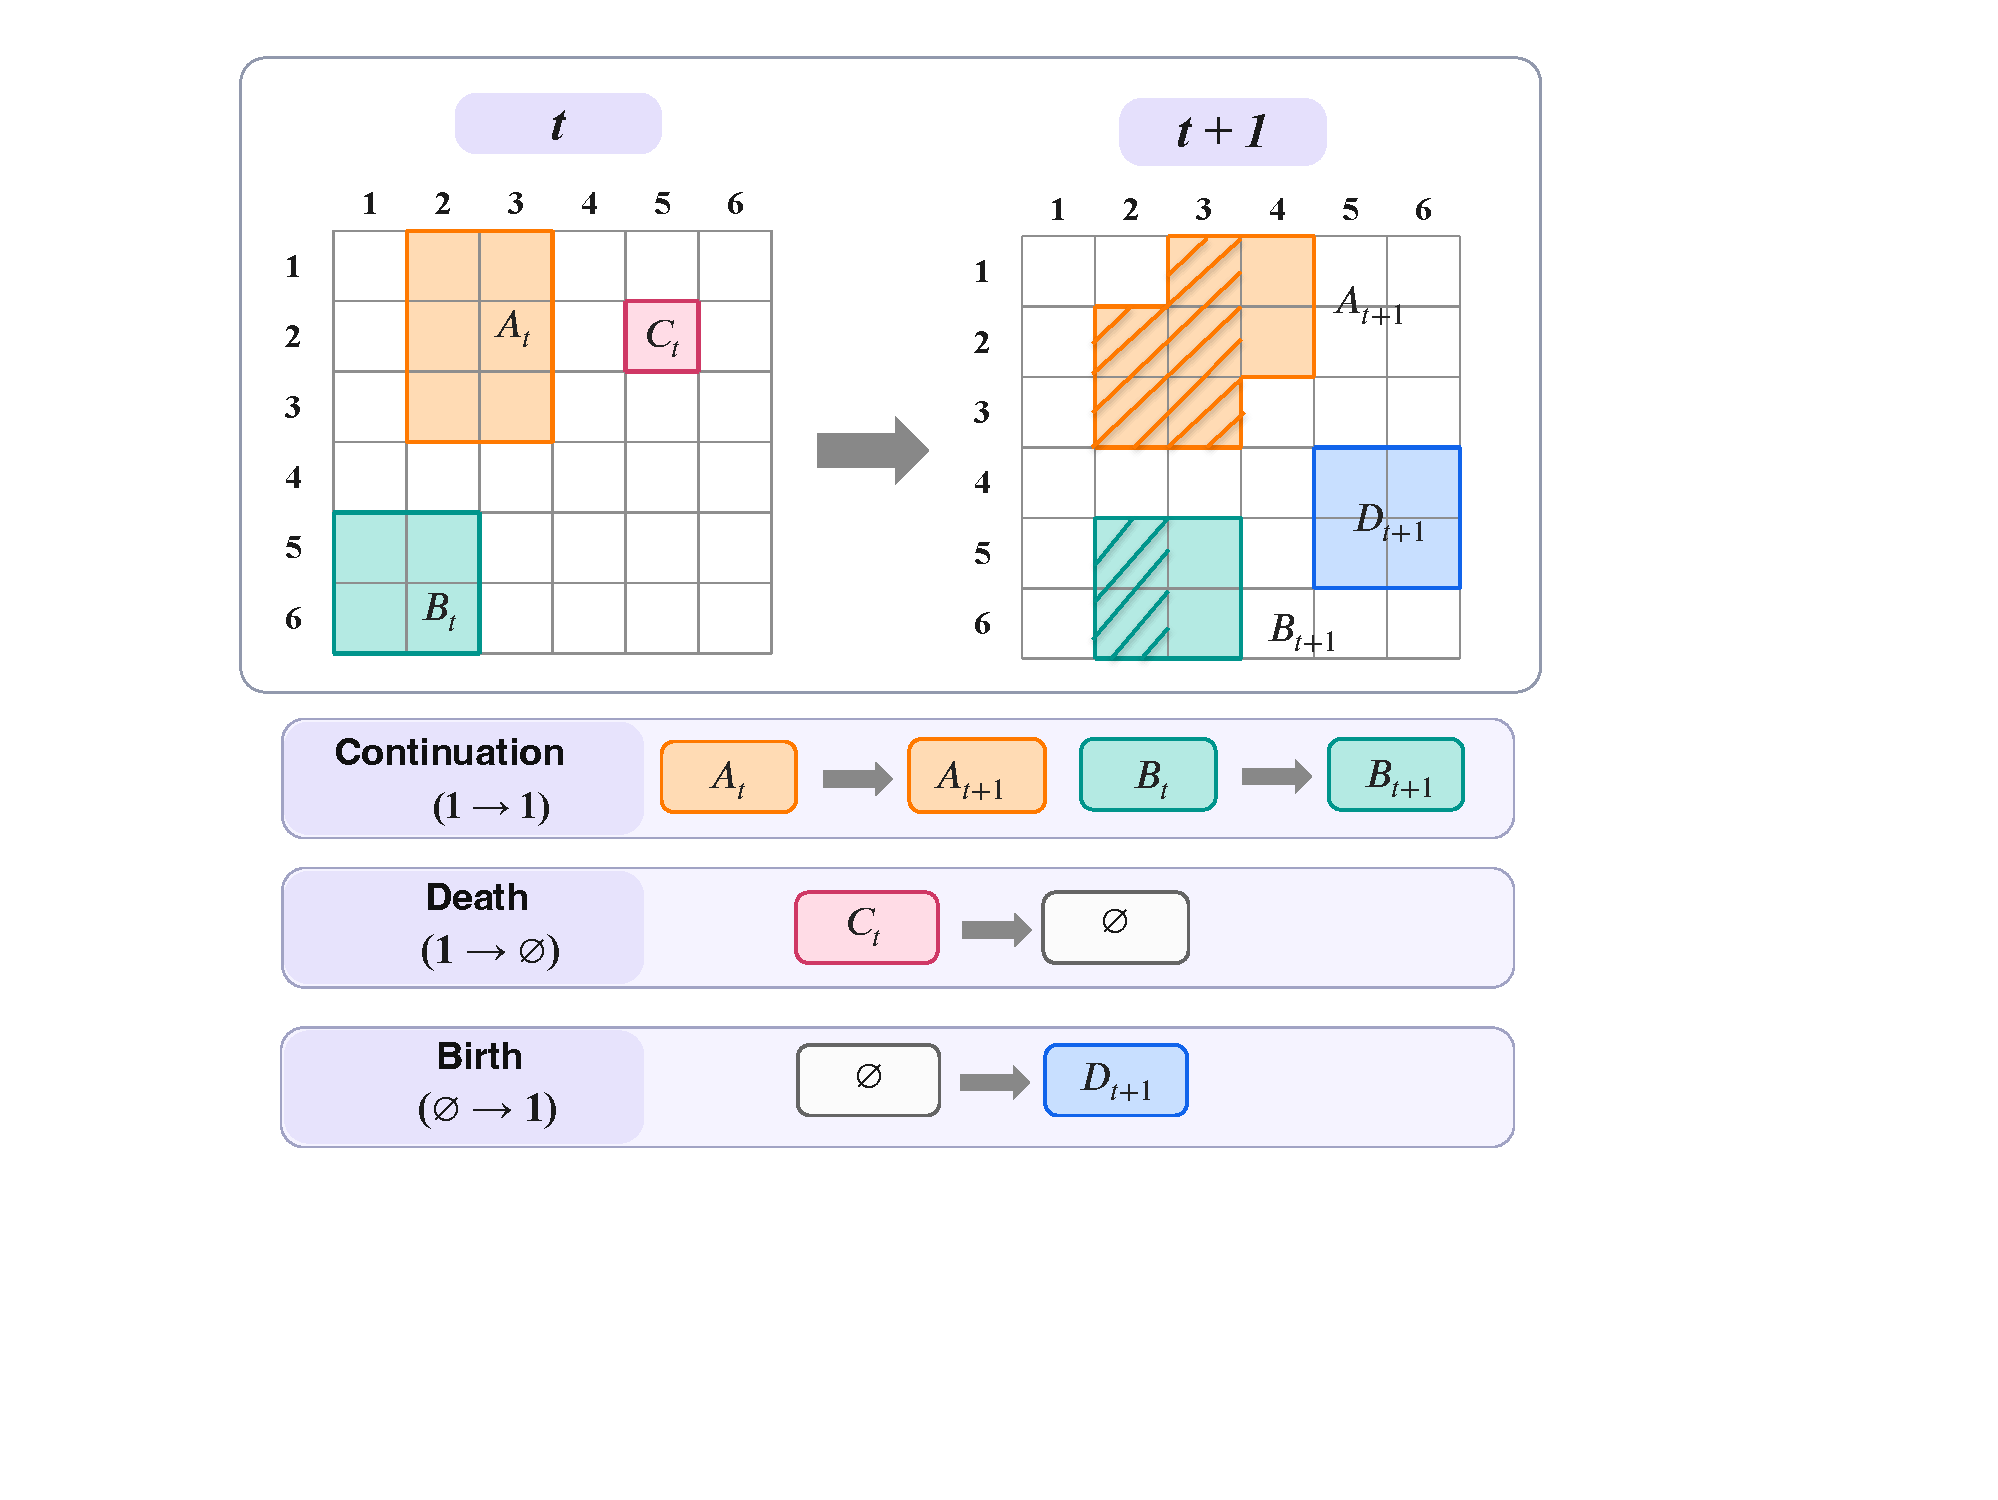
\includegraphics[width=\linewidth]{../figures/anchor_leaf_correspondence.pdf}
\caption{Overlap-based leaf correspondence. Hatching shows shared support samples. One-to-one maximum-overlap matching continues $A,B$, leaves $C_t$ unmatched and creates $D_{t+1}$. Birth/death denote matching states, not verified physical events.}
\label{fig:leaf_correspondence}
\end{figure}

\begin{figure}[tbp]
\centering
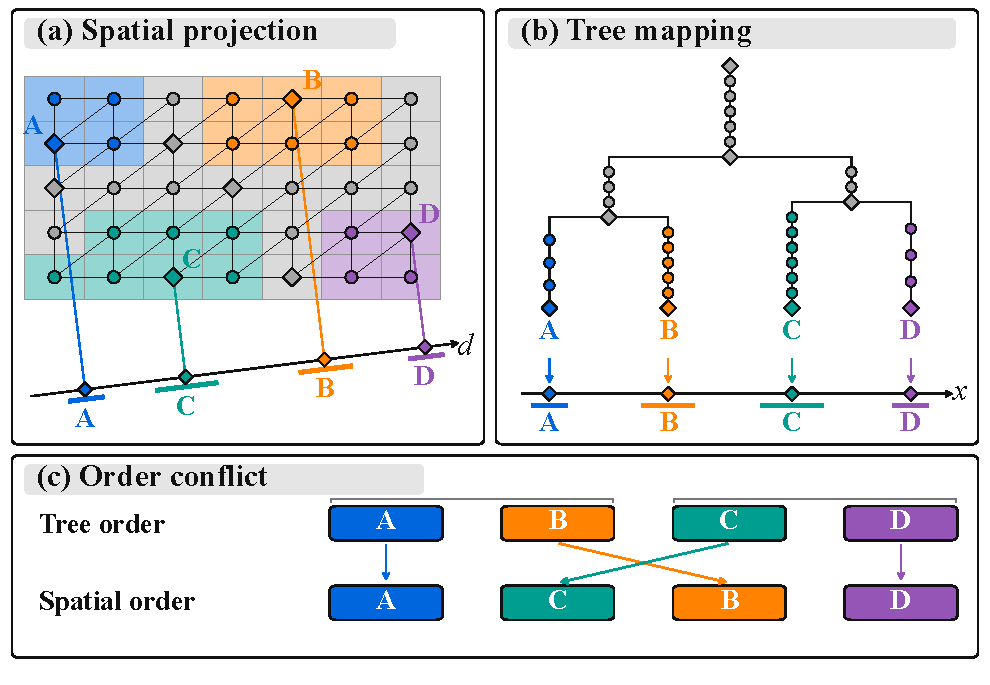
\includegraphics[width=\linewidth]{../figures/anchor_projection_conflict.pdf}
\caption{Synthetic reference--hierarchy conflict. (a) Extrema $A$--$D$ project onto a fixed direction; colors show leaf-arc supports. (b) The augmented merge tree of the same grid. (c) Spatial order interleaves sibling subtrees. Diamonds mark critical samples and circles regular samples; widths and mapped positions are schematic.}
\label{fig:projection_conflict}
\end{figure}

\begin{figure}[tbp]
\centering
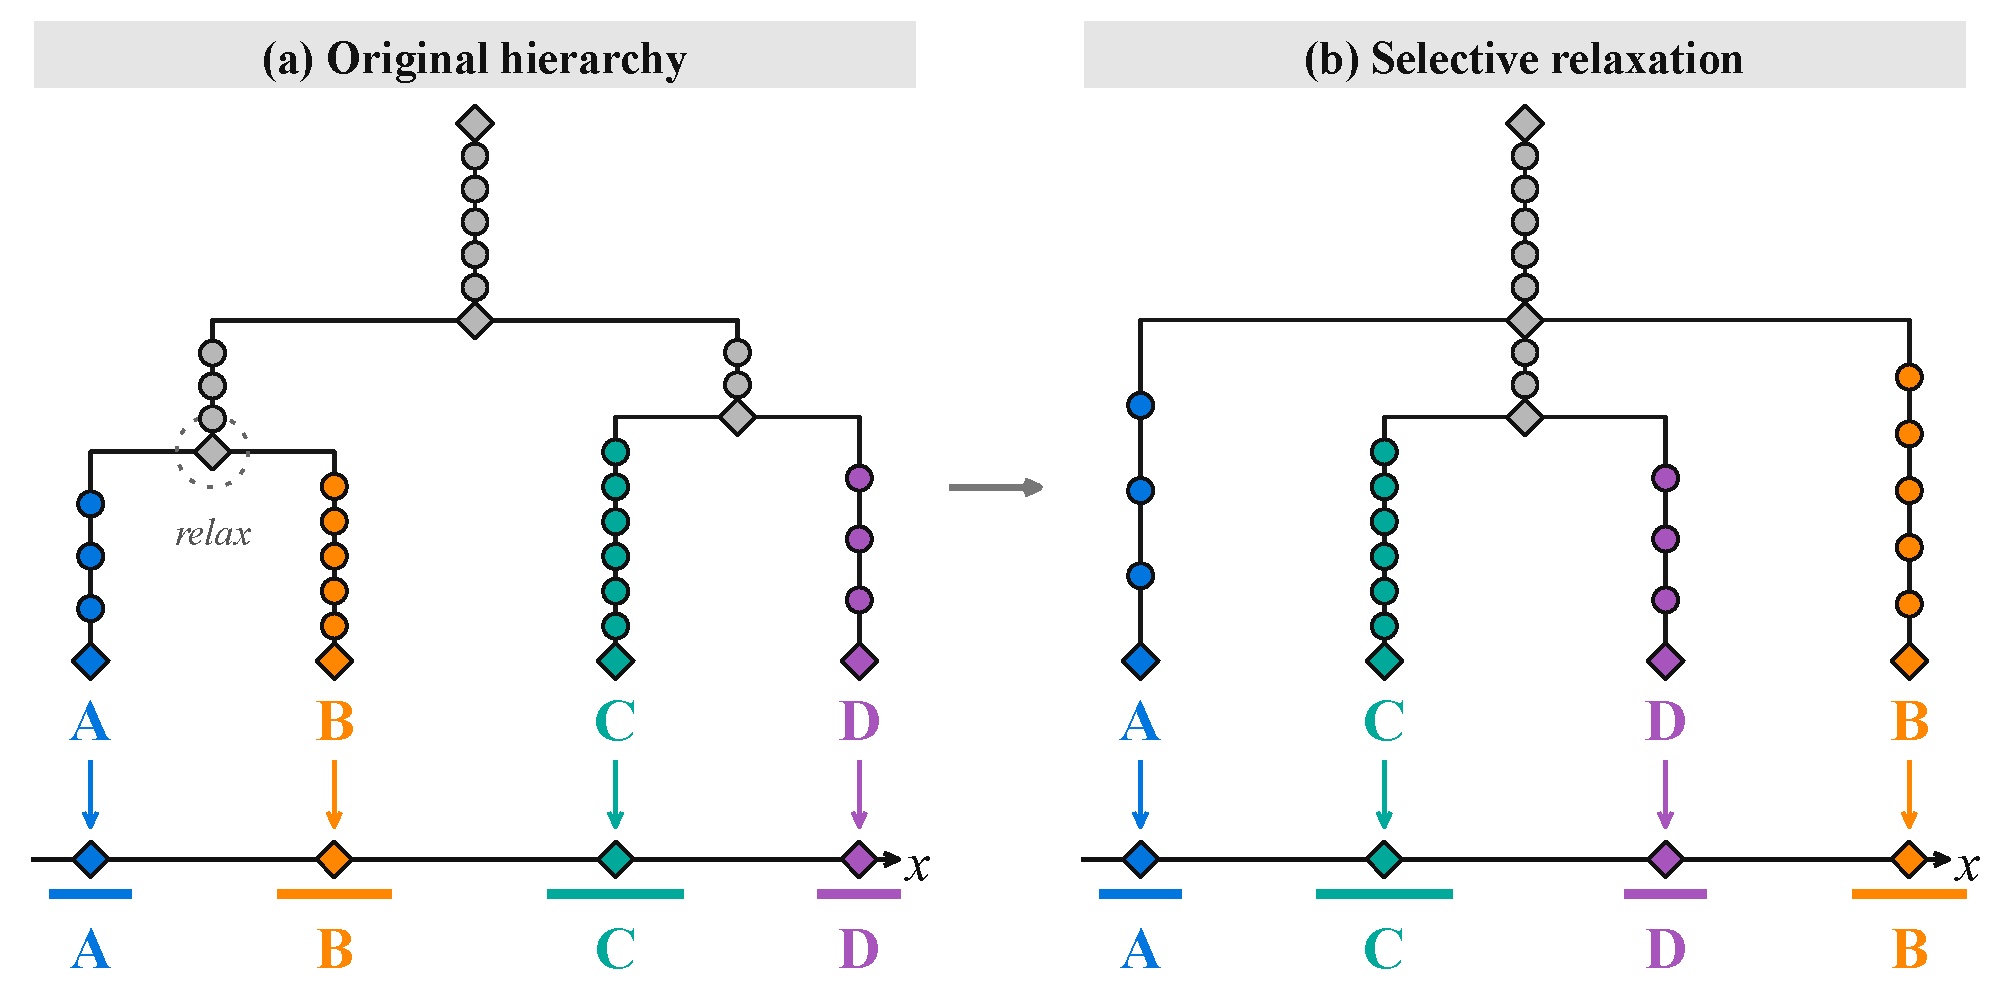
\includegraphics[width=\linewidth]{../figures/anchor_selective_relaxation.pdf}
\caption{Selective relaxation of the $A,B$ sibling constraint permits order $A,C,D,B$ while retaining subtree $C,D$. Diamonds mark critical nodes and circles regular samples; widths and spacing are schematic, not measured merge errors.}
\label{fig:selective_relaxation}
\end{figure}
